%%%%%%%%%%%%%%%%%%%%%%%%%%%%%%%%%%%%%%%%%%%%%%%%%%%%%%%%%%%%%%%%
%%%%%%%%%%%%%%%%%%%%%%%%%%%%%%%%%%%%%%%%%%%%%%%%%%%%%%%%%%%%%%%%
%%%%
%%%% This text file is part of the source of 
%%%% `Introduction to High-Performance Scientific Computing'
%%%% by Victor Eijkhout, copyright 2012
%%%%
%%%% This book is distributed under a Creative Commons Attribution 3.0
%%%% Unported (CC BY 3.0) license and made possible by funding from
%%%% The Saylor Foundation \url{http://www.saylor.org}.
%%%%
%%%%
%%%%%%%%%%%%%%%%%%%%%%%%%%%%%%%%%%%%%%%%%%%%%%%%%%%%%%%%%%%%%%%%
%%%%%%%%%%%%%%%%%%%%%%%%%%%%%%%%%%%%%%%%%%%%%%%%%%%%%%%%%%%%%%%%

One approach to  mitigating the difficulty of parallel programming
is the design of languages that offer explicit support for
parallelism. There are several approaches, and we will see some
examples.
\begin{itemize}
\item Some languages reflect the fact that many operations in
  scientific computing are data parallel
  (section~\ref{sec:data-parallel}). Languages such as \indexac{HPF}
  (section~\ref{sec:HPF}) have
  an \indexterm{array syntax}, where operations such addition of
  arrays can be expressed \n{A = B+C}. This syntax simplifies
  programming, but more importantly, it specifies operations at an
  abstract level, so that a lower level can make specific decision
  about how to handle parallelism. However, the data parallelism
  expressed in \ac{HPF} is only of the simplest sort, where the data
  are contained in regular arrays. Irregular data parallelism is
  harder; the \indexterm{Chapel} language (section~\ref{sec:Chapel})
  makes an attempt at addressing this.
\item Another concept in parallel languages, not necessarily
  orthogonal to the previous, is that of \acf{PGAS} model: there is only
  one address space (unlike in the MPI model), but this address space
  is partitioned, and each partition has affinity with a thread or
  process. Thus, this model encompasses both \ac{SMP} and distributed
  shared memory. A~typical \ac{PGAS} language, \indexac{UPC}, allows you
  to write programs that for the most part looks like regular C code.
  However, by indicating how the major arrays are distributed over
  processors, the program can be executed in parallel.
\end{itemize}

\Level 2 {Discussion}

Parallel languages hold the promise of making parallel programming
easier, since they make communication operations appear as simple
copies or arithmetic operations. However, by doing so they invite the
user to write code that may not be efficient, for instance by inducing
many small messages. 

\begin{figure}[ht]
  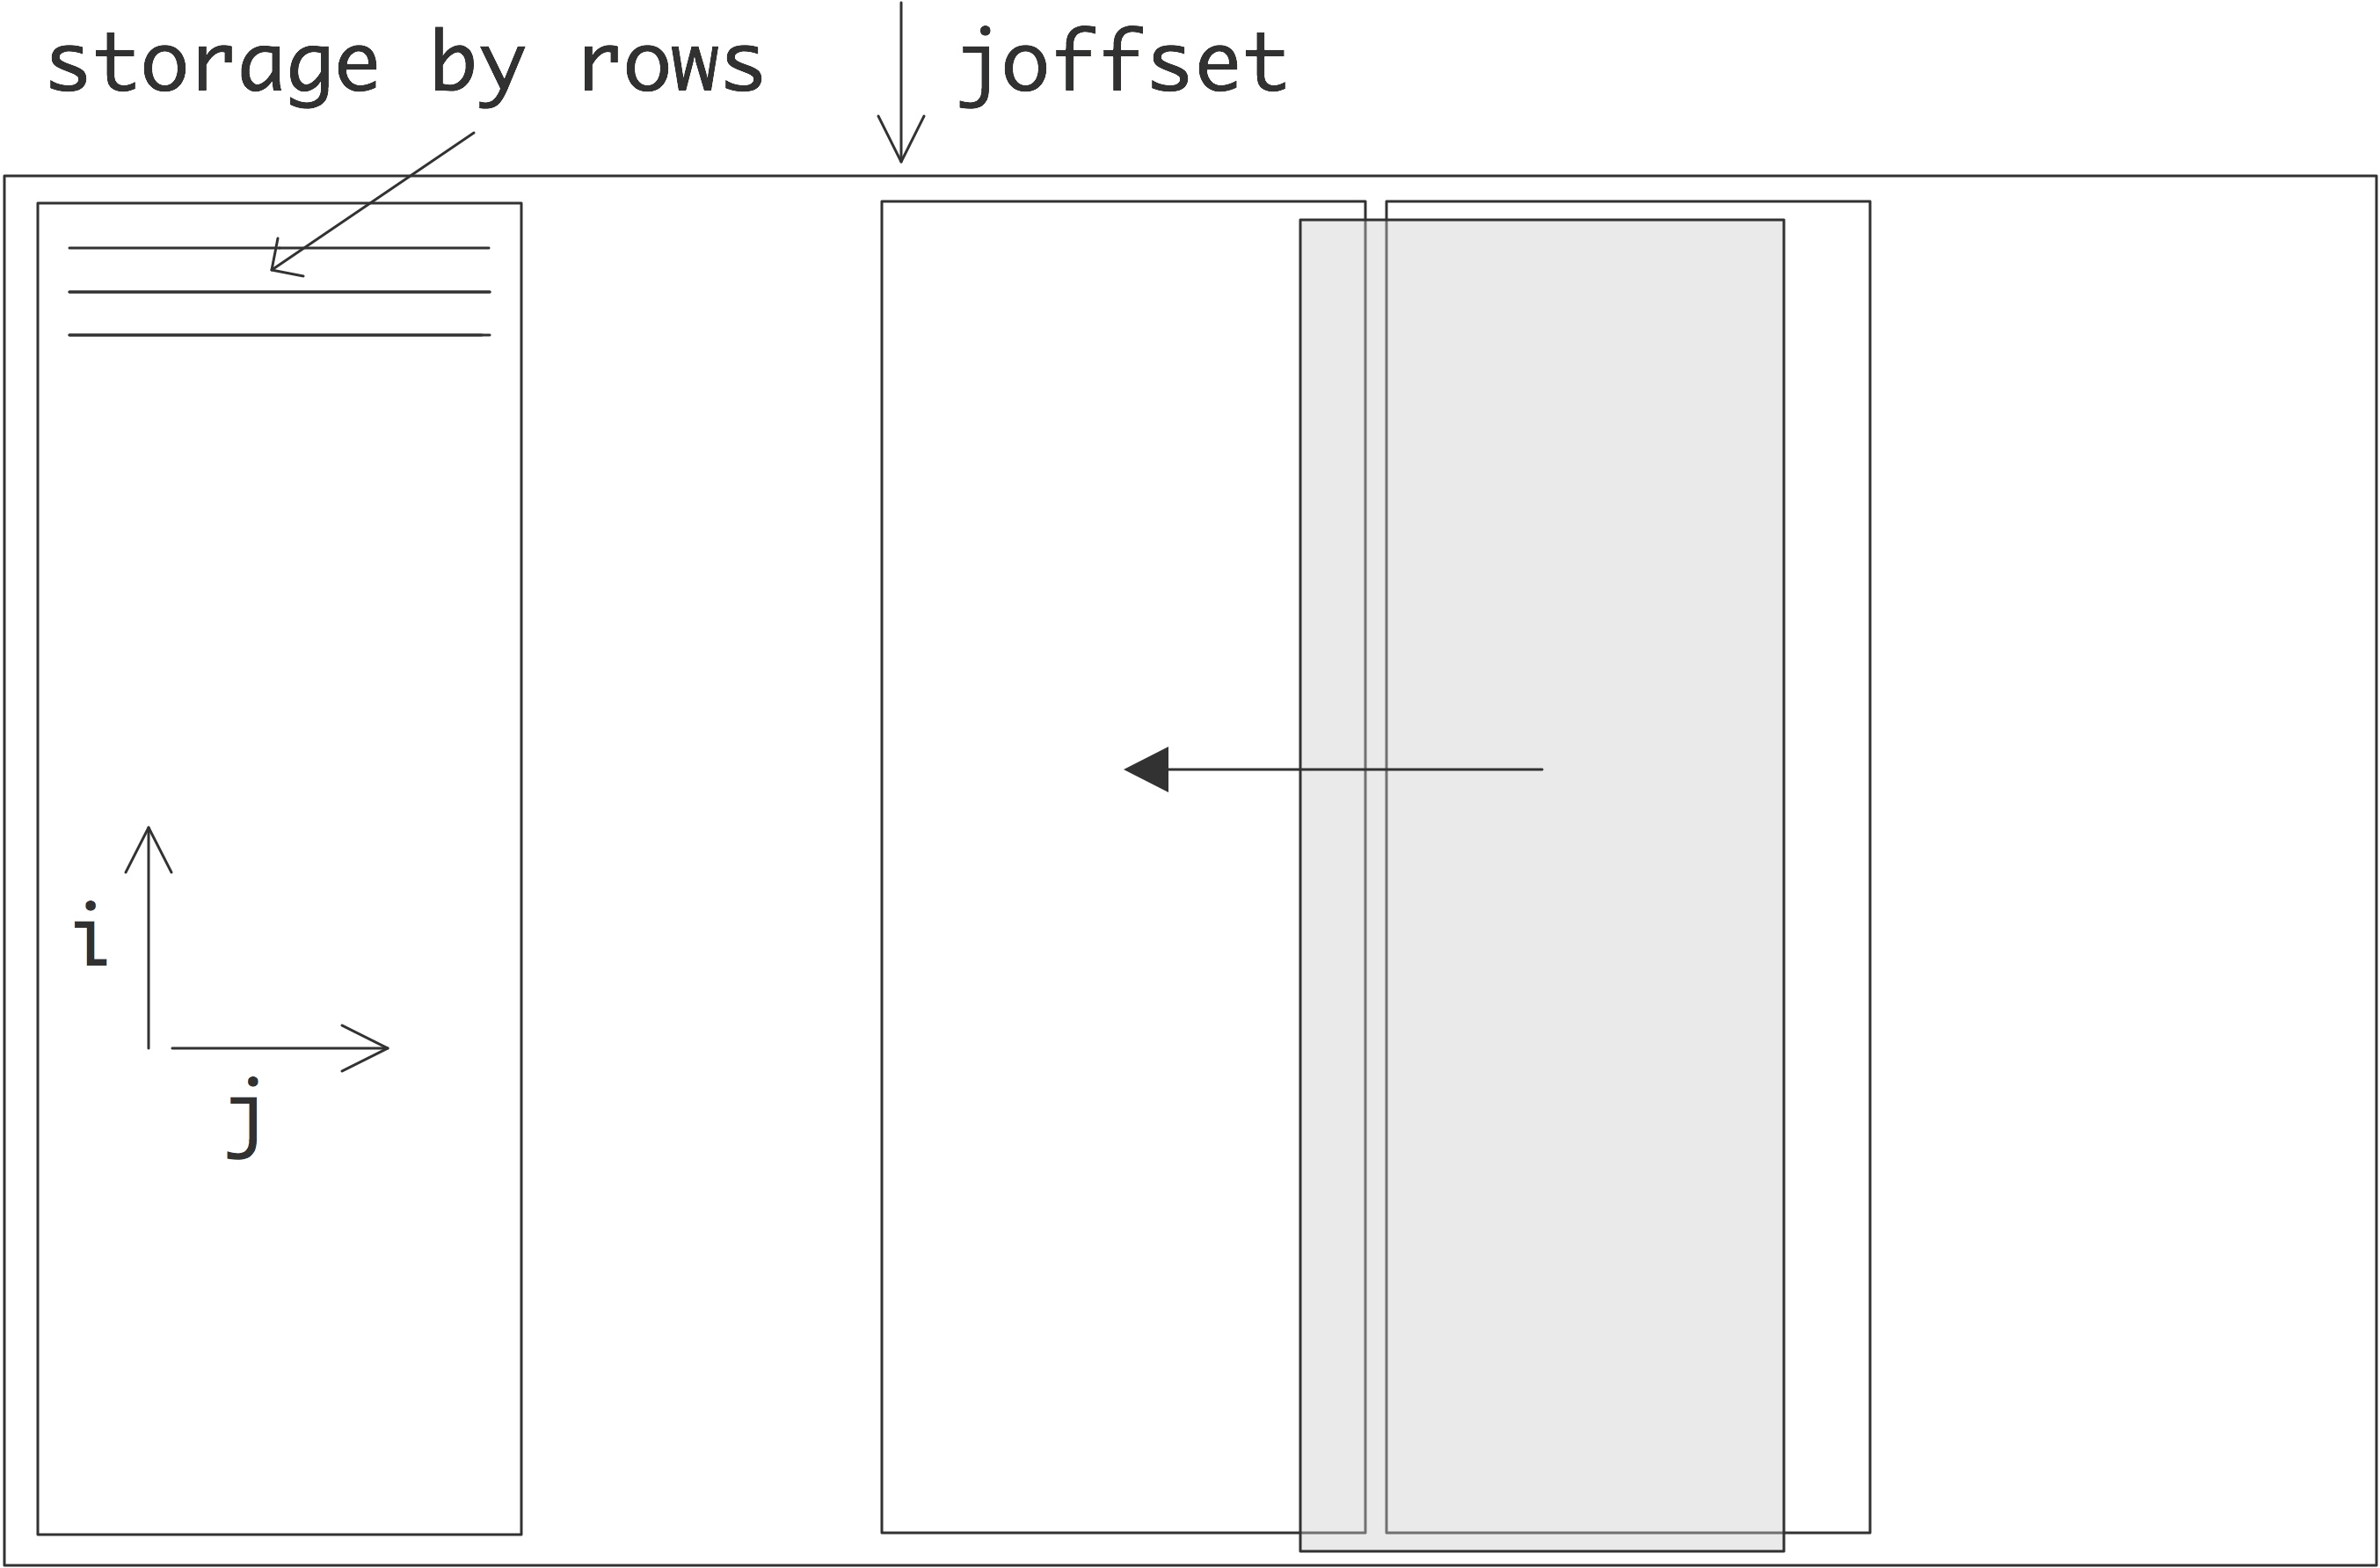
\includegraphics[scale=.12]{graphics/abshift}
  \caption{Data shift that requires communication}
  \label{fig:abshift}
\end{figure}
As an example, consider arrays \n{a,b} that have been horizontally
partitioned over the processors, and that are shifted (see figure~\ref{fig:abshift}):
\begin{verbatim}
for (i=0; i<N; i++)
  for (j=0; j<N/np; j++)
    a[i][j+joffset] = b[i][j+1+joffset]
\end{verbatim}
If this code is executed on a shared memory machine, it will be
efficient, but a naive translation in the distributed case will have a
single number being communicated in each iteration of the
\n{i}~loop. Clearly, these can be combined in a single buffer
send/receive operation, but compilers\index{compiler} are usually
unable to make this transformation. As a result, the user is forced
to, in effect, re-implement the blocking that needs to be done in an
MPI implementation:
\begin{verbatim}
for (i=0; i<N; i++)
  t[i] = b[i][N/np+joffset]
for (i=0; i<N; i++)
  for (j=0; j<N/np-1; j++) {
    a[i][j] = b[i][j+1]
    a[i][N/np] = t[i]
  }
\end{verbatim}

On the other hand, certain machines support direct memory copies
through global memory hardware. In that case, \ac{PGAS} languages can
be more efficient than explicit message passing, even with physically
distributed memory.

\Level 2 {Unified Parallel C}
\indexacstart{UPC}

\acf{UPC}~\cite{UPC:homepage} is an extension to the C~language.  Its
main source of parallelism is \indextermsub{data}{parallelism}, where
the compiler\index{compiler} discovers indepence of operations on
arrays, and assigns them to separate processors. The language has an
extended array declaration, which allows the user to specify whether
the array is partitioned by blocks, or in a
\emph{round-robin}\index{round-robin!storage assignment}
fashion.

The following program in \ac{UPC} performs a vector-vector addition.
\begin{verbatim}
//vect_add.c
#include <upc_relaxed.h>
#define N 100*THREADS
shared int v1[N], v2[N], v1plusv2[N];
void main() {
  int i;
  for(i=MYTHREAD; i<N; i+=THREADS)
    v1plusv2[i]=v1[i]+v2[i];
}
\end{verbatim}
The same program with an explicitly parallel loop construct:
\begin{verbatim}
//vect_add.c
#include <upc_relaxed.h>
#define N 100*THREADS
shared int v1[N], v2[N], v1plusv2[N];
void main()
{
  int i;
  upc_forall(i=0; i<N; i++; i)
    v1plusv2[i]=v1[i]+v2[i];
}
\end{verbatim}

\indexacend{UPC}

%\Level 2 {Titanium}
\index{Titanium} is comparable to \ac{UPC} in spirit, but based on Java rather
than on~C.

\Level 2 {High Performance Fortran}
\label{sec:HPF}
\indexacstart{HPF}

High Performance Fortran\footnote{This section quoted from Wikipedia}
(HPF) is an extension of Fortran 90 with constructs that support
parallel computing, published by the High Performance Fortran Forum
(HPFF). The HPFF was convened and chaired by Ken Kennedy of Rice
University. The first version of the HPF Report was published in 1993.

Building on the array syntax introduced in Fortran 90, HPF uses a data
parallel model of computation to support spreading the work of a
single array computation over multiple processors. This allows
efficient implementation on both SIMD and MIMD style
architectures. HPF features included:
\begin{itemize}
\item New Fortran statements, such as FORALL, and the ability to
  create PURE (side effect free) procedures;
\item The use of \indextermbus{compiler}{directives} for recommended
  distributions of array data;
\item Extrinsic procedure interface for interfacing to non-HPF
  parallel procedures such as those using message passing;
\item Additional library routines, including environmental inquiry,
  parallel prefix/suffix (e.g., 'scan'), data scattering, and sorting
  operations.
\end{itemize}
Fortran 95 incorporated several HPF capabilities.  While some vendors
did incorporate HPF into their compilers in the 1990s, some aspects
proved difficult to implement and of questionable use. Since then,
most vendors and users have moved to OpenMP-based parallel
processing. However, HPF continues to have
influence. For example the proposed BIT data type for the upcoming
Fortran-2008 standard contains a number of new intrinsic functions
taken directly from HPF.

\indexacend{HPF}

\Level 2 {Co-array Fortran}
\indexacstart{CAF}

\acf{CAF} is an extension to the Fortran 95/2003 language.
The main mechanism to support parallelism is an extension to the array
declaration syntax, where an extra dimension indicates the parallel
distribution. For instance, in
\begin{verbatim}
Real,dimension(100),codimension[*] :: X
Real :: Y(100)[*]
Real :: Z(100,200)[10,0:9,*]
\end{verbatim}
arrays \n{X,Y} have 100 elements on each processor.
Array \n{Z} behaves as if the available processors
are on a three-dimensional grid, with two sides specified 
and the third adjustable to accomodate the available processors.

Communication between processors is now done through copies along the
(co-)dimensions that describe the processor grid.
%% \begin{verbatim}
%%       COMMON/XCTILB4/ B(N,4)[*]
%%       SAVE  /XCTILB4/
%% C
%%       CALL SYNC_ALL( WAIT=(/IMG_S,IMG_N/) )
%%       B(:,3) = B(:,1)[IMG_S]
%%       B(:,4) = B(:,2)[IMG_N]
%%       CALL SYNC_ALL( WAIT=(/IMG_S,IMG_N/) )
%% \end{verbatim}
The Fortran 2008 standard includes co-arrays.

\indexacend{CAF}

\Level 2 {Chapel}
\label{sec:Chapel}
\index{Chapel|(}

Chapel~\cite{Chapel:homepage} is a new parallel programming
language\footnote{This section quoted from the Chapel homepage.}
being developed by Cray Inc. as part of the DARPA-led High
Productivity Computing Systems program (HPCS). Chapel is designed to
improve the productivity of high-end computer users while also serving
as a portable parallel programming model that can be used on commodity
clusters or desktop multicore systems. Chapel strives to vastly
improve the programmability of large-scale parallel computers while
matching or beating the performance and portability of current
programming models like MPI.

Chapel supports a multithreaded execution model via high-level
abstractions for data parallelism, task parallelism, concurrency, and
nested parallelism. Chapel's locale type enables users to specify and
reason about the placement of data and tasks on a target architecture
in order to tune for locality. Chapel supports global-view data
aggregates with user-defined implementations, permitting operations on
distributed data structures to be expressed in a natural manner. In
contrast to many previous higher-level parallel languages, Chapel is
designed around a multiresolution philosophy, permitting users to
initially write very abstract code and then incrementally add more
detail until they are as close to the machine as their needs
require. Chapel supports code reuse and rapid prototyping via
object-oriented design, type inference, and features for generic
programming.

Chapel was designed from first principles rather than by extending an
existing language. It is an imperative block-structured language,
designed to be easy to learn for users of C, C++, Fortran, Java, Perl,
Matlab, and other popular languages. While Chapel builds on concepts
and syntax from many previous languages, its parallel features are
most directly influenced by ZPL, High-Performance Fortran (HPF), and
the Cray MTA's extensions to C and Fortran.

Here is vector-vector addition in Chapel:
\begin{verbatim}
const BlockDist= newBlock1D(bbox=[1..m], tasksPerLocale=...);
const ProblemSpace: domain(1, 64)) distributed BlockDist = [1..m];
var A, B, C: [ProblemSpace] real;
forall(a, b, c) in(A, B, C) do
  a = b + alpha * c;
\end{verbatim}

\index{Chapel|)}

\Level 2 {Fortress}
\index{Fortress|(}

Fortress~\cite{Fortress:homepage} is a programming language developed
by Sun Microsystems.  Fortress\footnote{This section quoted from the
  Fortress homepage.} aims to make parallelism more tractable
in several ways. First, parallelism is the default. This is intended
to push tool design, library design, and programmer skills in the
direction of parallelism. Second, the language is designed to be more
friendly to parallelism. Side-effects are discouraged because
side-effects require synchronization to avoid bugs. Fortress provides
transactions, so that programmers are not faced with the task of
determining lock orders, or tuning their locking code so that there is
enough for correctness, but not so much that performance is
impeded. The Fortress looping constructions, together with the
library, turns "iteration" inside out; instead of the loop specifying
how the data is accessed, the data structures specify how the loop is
run, and aggregate data structures are designed to break into large
parts that can be effectively scheduled for parallel
execution. Fortress also includes features from other languages
intended to generally help productivity -- test code and methods, tied
to the code under test; contracts that can optionally be checked when
the code is run; and properties, that might be too expensive to run,
but can be fed to a theorem prover or model checker. In addition,
Fortress includes safe-language features like checked array bounds,
type checking, and garbage collection that have been proven-useful in
Java. Fortress syntax is designed to resemble mathematical syntax as
much as possible, so that anyone solving a problem with math in its
specification can write a program that can be more easily related to
its original specification.

\index{Fortress|)}

\Level 2 {X10}
\index{X10|(}

X10 is an experimental new language currently under development at
IBM\index{IBM} in collaboration with academic partners. The X10 effort
is part of the IBM PERCS project (Productive Easy-to-use Reliable
Computer Systems) in the DARPA program on High Productivity Computer
Systems. The PERCS project is focused on a hardware-software co-design
methodology to integrate advances in chip technology, architecture,
operating systems, compilers, programming language and programming
tools to deliver new adaptable, scalable systems that will provide an
order-of-magnitude improvement in development productivity for
parallel applications by 2010.

X10 aims to contribute to this productivity improvement by developing
a new programming model, combined with a new set of tools integrated
into Eclipse and new implementation techniques for delivering
optimized scalable parallelism in a managed runtime environment. X10
is a type-safe, modern, parallel, distributed object-oriented language
intended to be very easily accessible to Java(TM) programmers. It is
targeted to future low-end and high-end systems with nodes that are
built out of multi-core SMP chips with non-uniform memory hierarchies,
and interconnected in scalable cluster configurations. A member of the
Partitioned Global Address Space (PGAS) family of languages, X10
highlights the explicit reification of locality in the form of places;
lightweight activities embodied in async, future, foreach, and ateach
constructs; constructs for termination detection (finish) and phased
computation (clocks); the use of lock-free synchronization (atomic
blocks); and the manipulation of global arrays and data structures.

\index{X10|)}

\Level 2 {Linda}
\index{Linda|(}

As should be clear by now, the treatment of data is by far the most
important aspect of parallel programing, far more important than
algorithmic considerations. The programming system
\indexterm{Linda}~\cite{Gelernter85generativecommunication,Linda-CACM}, also called a
\indexterm{coordination language}, is designed to address the data
handling explicitly. Linda is not a language as such, but can, and has
been, incorporated into other languages.

The basic concept of Linda is \indexterm{tuple space}: data is added
to a pool of globally accessible information by adding a label to
it. Processes then retrieve data by their label, and without needing to
know which processes added them to the tuple space.

Linda is aimed primarily at a different computation model than is
relevant for \indexac{HPC}: it addresses the needs of
asynchronous communicating processes. However, is has been used for
scientific computation~\cite{Deshpande92efficientparallel}. For
instance, in parallel simulations of the heat equation
(section~\ref{sec:heateq}), processors can write their data into tuple
space, and neighbouring processes can retrieve their \indexterm{ghost
  region} without having to
know its provenance. Thus, Linda becomes one way of implementing
\indexterm{one-sided communication}.

\index{Linda|)}

\Level 2 {The Global Arrays library}
\index{Global Arrays|(}

The Global Arrays library (\url{http://www.emsl.pnl.gov/docs/global/})
is another example of \indexterm{one-sided communication}, and in fact
it predates MPI. This library has as its prime data structure
\indexterm{cartesian product} arrays\footnote{This means that if the
  array is three-dimensional, it can be described by three integers
  $n_1,n_2,n_3$, and each point has a coordinate $(i_1,i_2,i_3)$ with
  $1\leq i_1\leq n_1$ et cetera.}, distributed over a processor grid
of the same or lower dimension. Through library calls, any processor
can access any sub-brick out of the array in either a \n{put} or
\n{get} operation. These operations are non-collective. As with any
one-sided protocol, a barrier sync is necessary to ensure completion
of the sends/receives.

\index{Global Arrays|)}

